\subsection{Agen Penguji dan Alur Pengujian}

Selama pengujian, akan ada banyak agen yang dijalankan untuk menyimulasikan perilaku pengguna mulai dari \textit{login} hingga pemesanan berhasil atau gagal. Agen ini juga akan mencatat latensi dan waktu yang dibutuhkan untuk menyelesaikan setiap tahapan saat pemesanan. Berikut adalah gambaran diagram alur agen penguji:

Pertama-tama, agen akan melakukan aksi \textit{login} lalu menunggu hingga penjualan dibuka. Setiap agen sudah diatur untuk memiliki kategori tiket tertentu yang ingin dibeli beserta jumlahnya. Saat sudah dibuka, agen akan mengambil data ketersediaan tiket, memilih \textit{seat} dan jumlah tiket yang ingin dipesan, lalu melakukan proses pembelian. Apabila pesanan gagal dibuat, agen akan memanggil ulang data ketersediaan tiket, lalu mencoba memesan lagi sampai tidak ada tiket tersedia yang sesuai dengan kebutuhan agen. Apabila pesanan berhasil dibuat, agen akan melakukan pembayaran. Pembayaran yang dilakukan agen dibuat agar memiliki kemungkinan kecil untuk gagal. Setelah pembayaran terverifikasi, agen akan memanggil \textit{endpoint} untuk memeriksa status pesanan yang sudah dibuat. Apabila pesanan sudah terkonfirmasi, alur pembelian untuk agen tersebut dianggap selesai.

\begin{figure}[htbp]
    \centering
    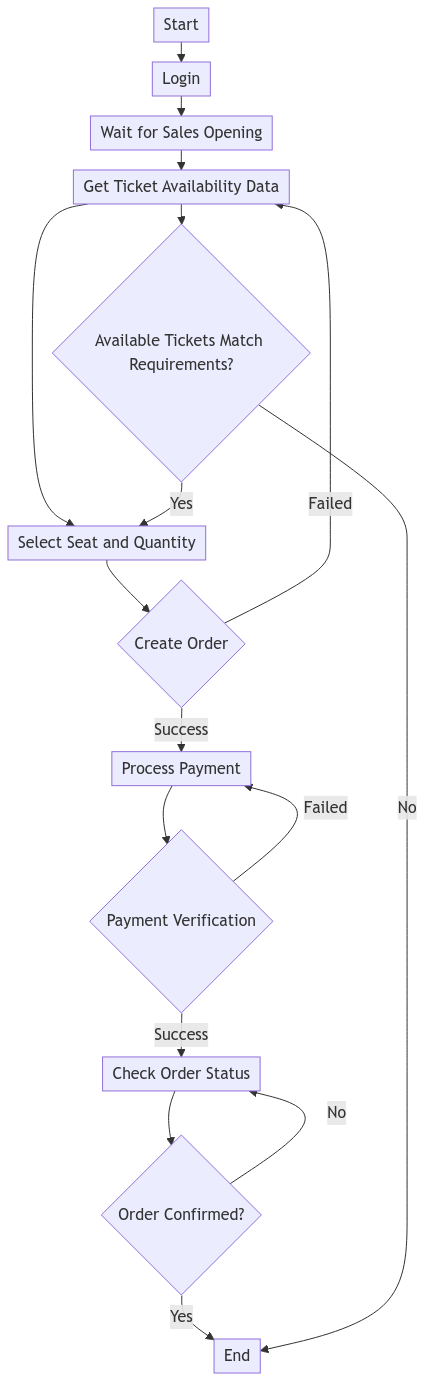
\includegraphics[width=0.4\textwidth]{resources/appendix/flow-agent.png}
    \caption{Alur Perilaku Agen Penguji}
    \label{fig:agent-flow}
\end{figure}